\documentclass[11pt]{a0poster}

\usepackage{url}
\usepackage{graphicx}
\usepackage[usenames,dvipsnames]{color}
\usepackage[margin=0in]{geometry}
\usepackage{xcolor}
\usepackage{graphicx}
\usepackage{amsmath}

\widowpenalty=500
\clubpenalty=500
\fboxsep=0pt

\renewcommand*{\familydefault}{\sfdefault}

\date{}

\begin{document}

\begin{minipage}{0.887\linewidth}
\vspace{75pt}
\hspace{92pt}
\color{Blue}
{\fontsize{2.5cm}{1em} \textbf{ADAM Enables Distributed Analyses Across Large Scale Genomic Datasets}}

%\vspace{0pt}
\hspace{92pt}
\fontsize{1cm}{1em}
Frank~Austin~Nothaft$^{1,2,\star}$, Arun~Ahuja$^3$, Timothy~Danford$^{1,4}$,
Michael~Heuer$^1$, Jey~Kottalam$^1$, Matt~Massie$^1$, Audrey~Musselman-Brown$^5$,
Beau~Norgeot$^{5,6}$, Ravi~Pandya$^7$, Justin~Paschall$^1$, Hannes~Schmidt$^5$,

\hspace{100pt} Eric~Tu$^1$, Ryan~Williams$^3$,
Carl~Yeksigian$^4$, Michael~Linderman$^3$, Jeff~Hammerbacher$^3$,
\textbf{Benedict~Paten}$^{5,\star}$, Uri~Laserson$^{3,9}$, Gaddy Getz$^{10}$,
David~Haussler$^5$, Anthony~D.~Joseph$^1$, David~A.~Patterson$^{1,2}$

\hspace{100pt}
$^1$AMPLab, University of California, Berkeley, CA,
$^2$ASPIRE Lab, University of California, Berkeley, CA,
$^3$Icahn School of Medicine at Mount Sinai, New York, NY,

\hspace{100pt}
$^4$Tamr, Inc., Cambridge, MA,
$^5$Genome Informatics Lab, University of Californa, Santa Cruz, CA,
$^6$Pharmaceutical Science and Pharmacogenomics, University of California, San Francisco, CA

\hspace{100pt}
$^7$Microsoft Research, Redmond, WA,
$^8$GenomeBridge, Cambridge, MA,
$^9$Cloudera, Inc., San Francisco, CA,
$^{10}$The Broad Institute of MIT and Harvard, Cambridge, MA

\hspace{100pt}
\fontsize{1cm}{1em}
$\star =$ \{fnothaft@berkeley.edu, benedict@soe.ucsc.edu\}
\vspace{75pt}
\end{minipage}
\begin{minipage}{0.113\linewidth}
\includegraphics[scale=0.6]{ucseal_540_139.pdf}
\end{minipage}

{\color{Blue}\noindent\makebox[\linewidth]{\rule{\paperwidth}{30pt}}}

\noindent\colorbox{Yellow}{
\begin{minipage}[t][2045pt][t]{\linewidth}

\noindent\begin{minipage}{0.025\linewidth}
\hfill
\pagebreak
\end{minipage}
\begin{minipage}{0.3\linewidth}
\vspace{75pt}
\colorbox{Blue}{
\begin{minipage}{\linewidth}
\vspace{25pt}
\begin{center}
\Huge \bf \color{White} Background
\end{center}
\vspace{10pt}
\end{minipage}
}
\colorbox{White}{
\begin{minipage}[t][600pt][t]{\linewidth}
\color{Blue}
\vspace{20pt}
\LARGE Currently, it is hard to write analyses that scan across large genomic
datasets:

\vspace{33pt}
\begin{itemize}
\item High performance computing systems have poor I/O perf.
\item Users frequently struggle with inconsistent file formats
\item Current computational model is too low level
\end{itemize}
\vspace{33pt}

ADAM is a framework that allows for the efficient parallelism of genomic queries
using Apache Spark. ADAM outperforms traditional tools on a single node, and
can scale to hundreds of nodes.
\hfill
\pagebreak
\end{minipage}
}

\vspace{75pt}
\colorbox{Blue}{
\begin{minipage}{\linewidth}
\vspace{25pt}
\begin{center}
\Huge \bf \color{White} Performance
\end{center}
\vspace{10pt}
\end{minipage}
}
\colorbox{White}{
\begin{minipage}[t][1020pt][t]{\linewidth}
\color{Blue}
\vspace{20pt}
\LARGE
\begin{itemize}
\item Compared to GATK, Picard, samtools, and Sambamba
\item Evaluated core processing steps on 234GB NA12878 dataset
\item Evaluated using 1 \texttt{i2.8xlarge} and 32--128 \texttt{r3.2xlarge} instances on EC2
\end{itemize}
\begin{center}
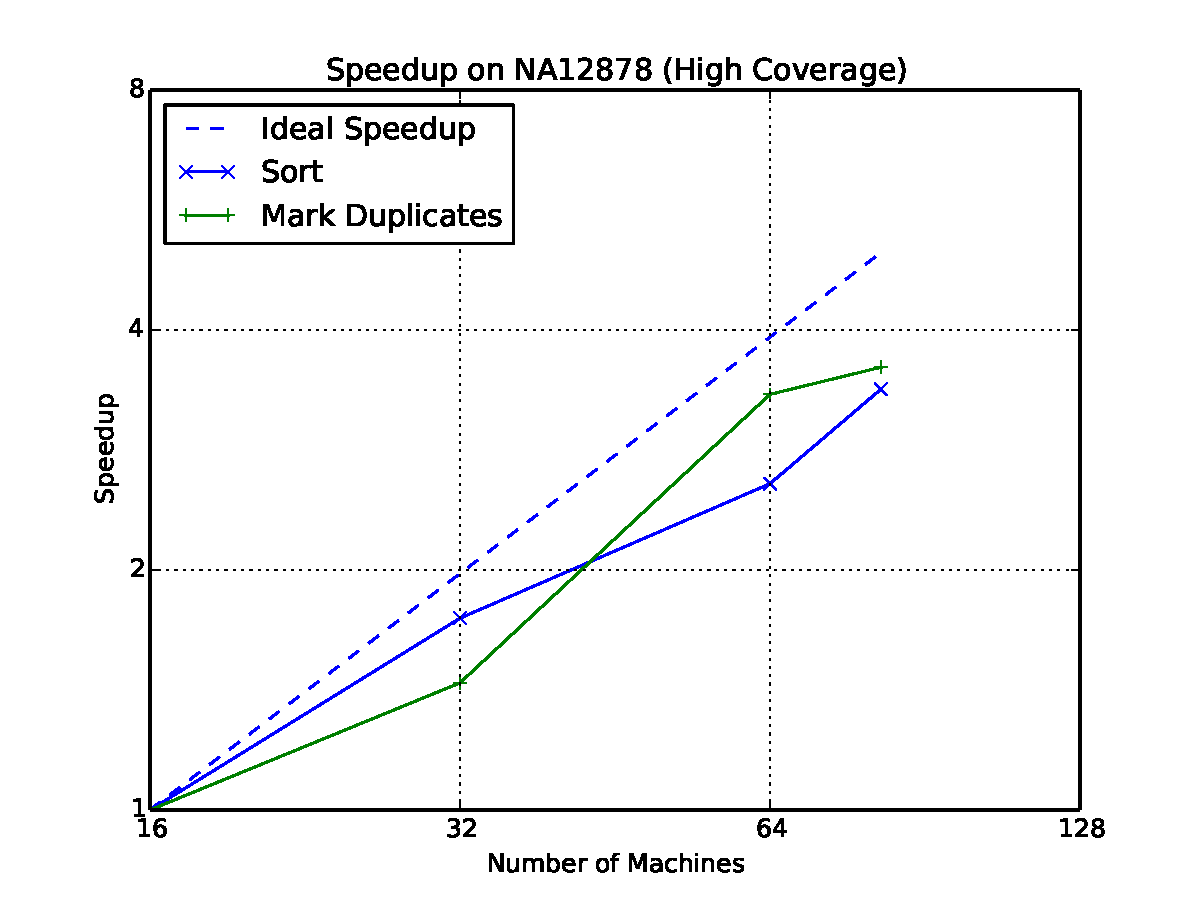
\includegraphics[width=0.83\linewidth]{speedup_na12878.pdf}
\end{center}
\small See detailed numbers in Nothaft et al, ``Rethinking data-intensive science using scalable analytics systems.''
In Proceedings of the International Conference on Management of Data, May 2015 (SIGMOD '15).
\pagebreak
\end{minipage}
}
\pagebreak
\end{minipage}
\begin{minipage}{0.03\linewidth}
\hfill
\pagebreak
\end{minipage}
\begin{minipage}{0.6\linewidth}

\vspace{70pt}
\colorbox{Blue}{
\begin{minipage}[t]{\linewidth}
\vspace{30pt}
\begin{center}
\Huge \bf \color{White} Architecture
\end{center}
\vspace{17pt}
\end{minipage}
}
\colorbox{White}{
\begin{minipage}[t][1000pt][t]{\linewidth}
\begin{minipage}{0.005\linewidth}
\hfill
\pagebreak
\end{minipage}
\begin{minipage}{0.32\linewidth}
\vspace{10pt}
\LARGE
\color{Blue}
ADAM uses a decomposed stack model. This has important benefits:
\begin{itemize}
\item Queries are programmed against a schema. The user doesn't need to know the
format of data on disk, or where data is physically stored.
\item ADAM builds upon Apache Spark's RDD model. RDDs are parallel arrays,
and all transformations to an RDD run in parallel.
\item Most systems use lower level abstractions, like an iterator over the genome.
ADAM queries are written with higher level primitives: duplicate marking maps to
a \texttt{groupBy}, finding overlapping genomic objects is implemented as an
optimized parallel join.
\end{itemize}
\end{minipage}
\begin{minipage}{0.005\linewidth}
\hfill
\pagebreak
\end{minipage}
\begin{minipage}{0.64\linewidth}
\vspace{30pt}
\hspace{100pt}
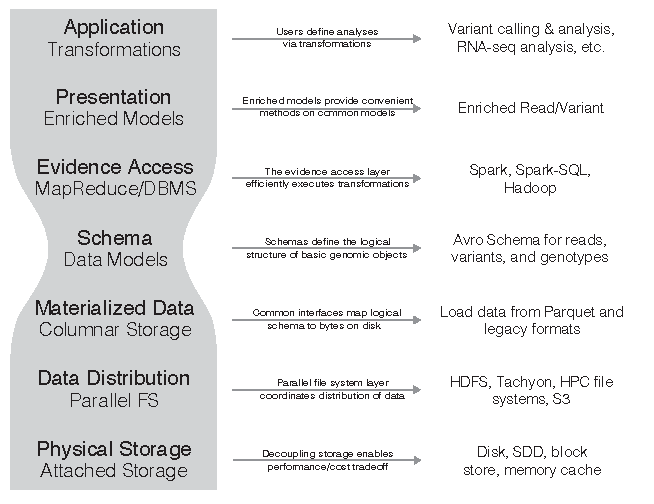
\includegraphics[width=0.95\linewidth]{expanded-stack-2.pdf}
\end{minipage}
\pagebreak
\end{minipage}
}

\vspace{75pt}
\begin{minipage}{\linewidth}
\colorbox{Blue}{
\begin{minipage}[t]{\linewidth}
\vspace{30pt}
\begin{center}
\Huge \bf \color{White} Accuracy Against GATK Best Practices
\end{center}
\vspace{17pt}
\end{minipage}
}
\colorbox{White}{
\begin{minipage}[t][590pt][t]{\linewidth}
\begin{minipage}{0.005\linewidth}
\hfill
\pagebreak
\end{minipage}
\begin{minipage}{0.55\linewidth}
\LARGE
\color{Blue}
\begin{itemize}
\item We evaluated ADAM by replacing the GATK ``Best Practices'' pre-processing
stages with an ADAM based reimplementation
\item GATK was run on a single \texttt{i2.8xlarge} node, ADAM was run on 16
\texttt{r3.4xlarge} nodes
\item The ADAM-based pipeline is $3.55\times$ faster, and $2\times$ cheaper
\item The two pipelines generate statistically equivalent variant calls
\end{itemize}

During this process, we identified two bugs in the GATK/Picard.
Both of these issues are caused by sort order invariants necessitated by
programming at a lower level of abstraction.
\end{minipage}
\begin{minipage}{0.03\linewidth}
\hfill
\pagebreak
\end{minipage}
\begin{minipage}{0.4\linewidth}
\color{Blue}
\begin{center}
\end{center}
\color{Blue}
\begin{center}
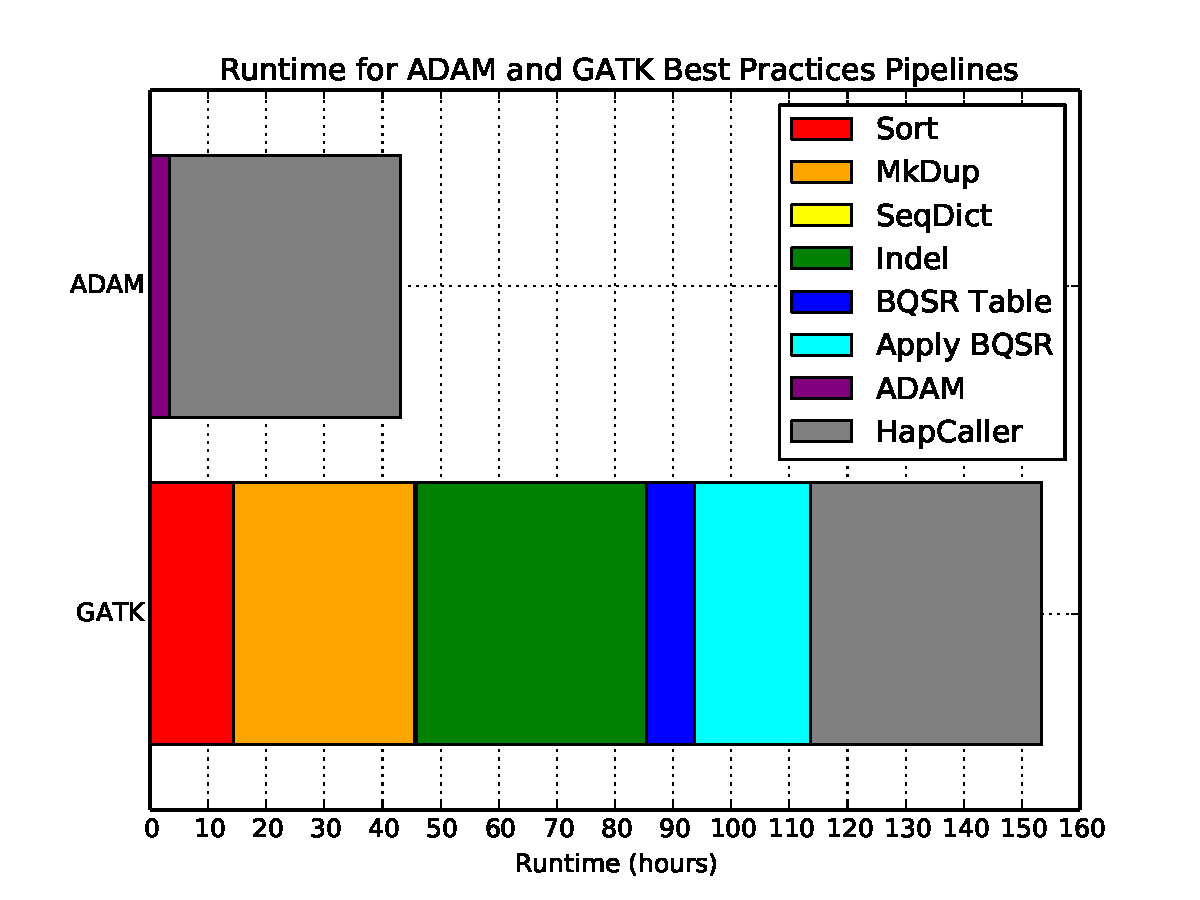
\includegraphics[width=0.9\linewidth]{perf.pdf}
\end{center}
\end{minipage}
\end{minipage}
}
\end{minipage}
\end{minipage}
\end{minipage}
}

\end{document}
